\documentclass[11pt]{beamer}
\usepackage[utf8]{inputenc}
%\usepackage[frenchb]{babel}
\usepackage{graphicx}
%\usepackage{textpos}
\usepackage{textcomp}

\usetheme{Berlin}%Berlin
\useinnertheme{rounded}
\usecolortheme{beaver}%beaver

\makeatletter
\beamer@theme@subsectionfalse
\makeatother 

\title{PRÁCTICA METRO MONTERREY}
\author{Genevieve CIRERA, \\Jaime LABIAGA, \\Juan Francisco SALAMANCA CARMONA}
%\subtitle{Soutenance intermédiaire d'apprentissage}
\date{\textit{3 de junio 2014}}


\begin{document}

\begin{frame}
\titlepage
\end{frame}

% --------- Sommaire -----------
%\AtBeginSection[]{
%  \begin{frame}{Sumario}
%  \small \tableofcontents[currentsection, hideothersubsections]
%  \end{frame} 
%}
% ------------------------------

% ----- Presentacion ------
\section{Presentación}

\subsection*{Definici\'on}
\begin{frame}{Objetivo}
	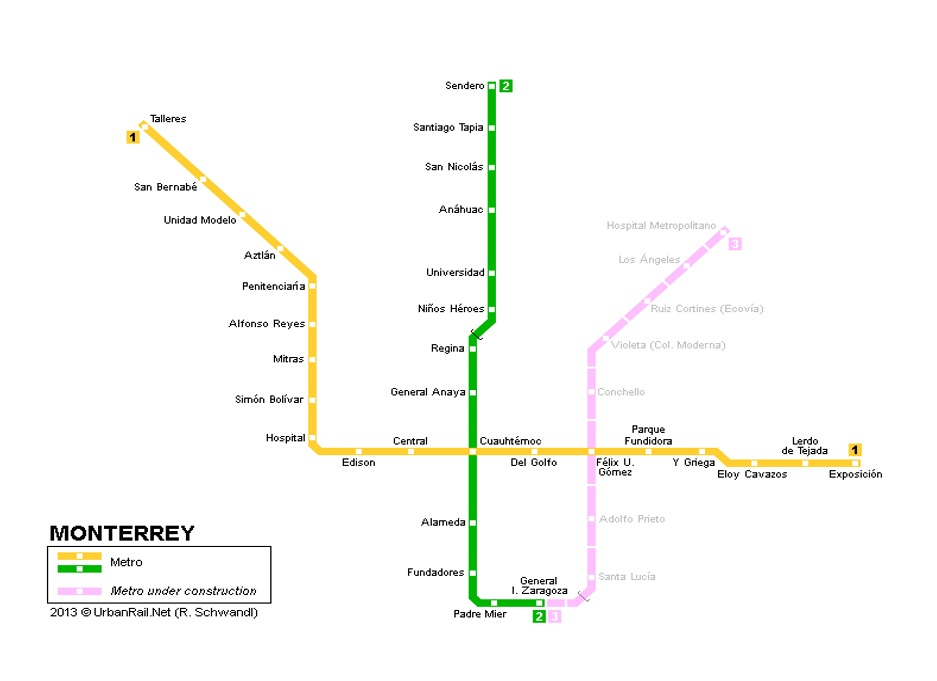
\includegraphics[width=0.9\textwidth]{images/MapaMetroMonterrey.jpg}
\end{frame}

\begin{frame}{MEDIOS UTILIZADOS}
\begin{itemize}
\item Algoritmo A*
\item Java
\item Interfaz : Swing
\item Datos : .txt
\end{itemize}
\end{frame}

\begin{frame}{Estructura : MVC}
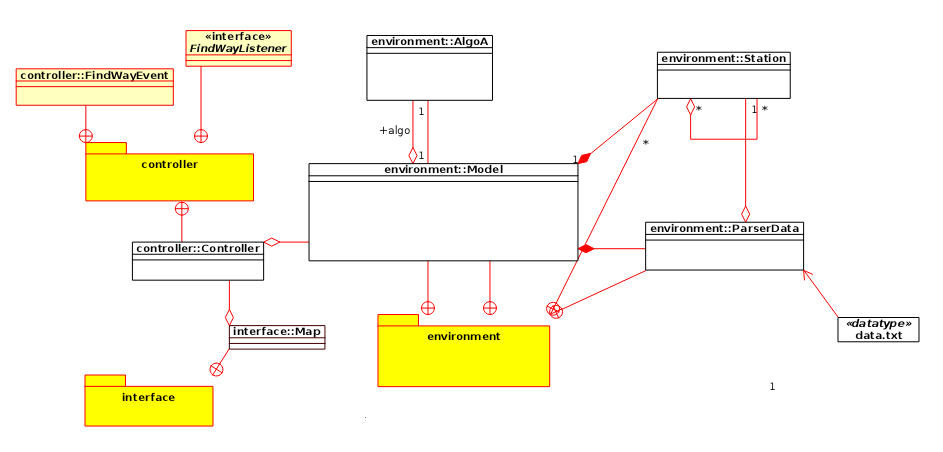
\includegraphics[width=1.1\textwidth]{images/classDiagram.png}
\end{frame}

\begin{frame}{Recogida de datos}
\begin{itemize}
\item Declaración de las estaciones
\end{itemize}
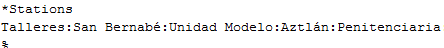
\includegraphics[width=0.9\textwidth]{images/datosDecl.png}
\\
\begin{itemize}
\item Distancias
\end{itemize}
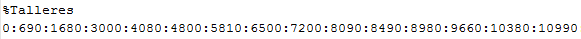
\includegraphics[width=1\textwidth]{images/datosDist.png}
\\
\begin{itemize}
\item Vínculos
\end{itemize}
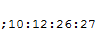
\includegraphics[width=0.4\textwidth]{images/datosVinc.png}
\end{frame}
%%%%%%%%%%%%%%%%%%%%%%%%%%%Clases%%%%%%%%%%%%%%%%%%%
\section{Clases}
\subsection*{Definici\'on}
\begin{frame}{Environment}
Dividida en cinco clases
\begin{itemize}
\item AlgoA
\item Main
\item Station
\item ParserData
\item Model
\end{itemize}
\end{frame}

\begin{frame}{ENVIRONMENT.Model}
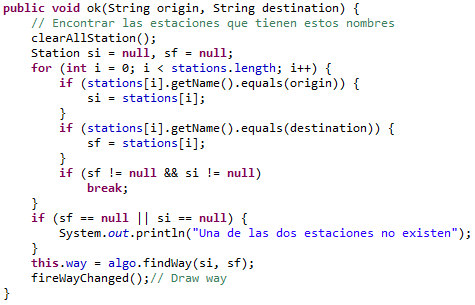
\includegraphics[width=1\textwidth]{images/ok.png}
\end{frame}

\begin{frame}{ENVIRONMENT.Find}
Llamado por el Model

\includegraphics[width=1\textwidth]{images/findWay.png}
\vspace{0.5cm}
Llamado recursivamente\\

\includegraphics[width=0.6\textwidth]{images/find.png}
\vspace{0.5cm}
\\
Criterio stop\\
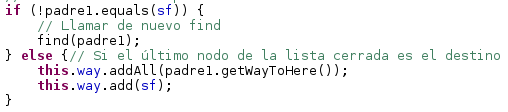
\includegraphics[width=0.8\textwidth]{images/findStop.png}
\end{frame}

\begin{frame}{ENVIRONMENT. AlgoA}
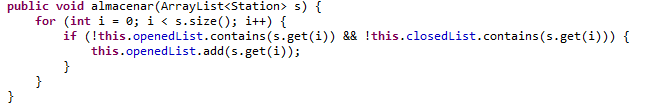
\includegraphics[width=1\textwidth]{images/almacenar.png}
\\
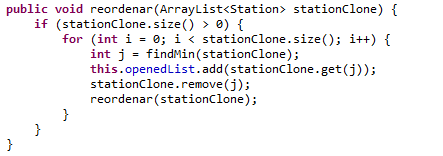
\includegraphics[width=0.7\textwidth]{images/reordenar.png}
\\
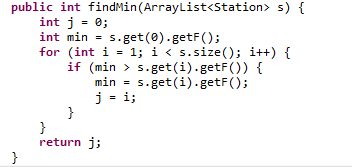
\includegraphics[width=0.6\textwidth]{images/findmin.png}
\end{frame}

%%%%%%%%%%%%%%%%%%%%%%%%%Interfaz y problemas%%%%%%%%%%%%%%
\section{Interfaz y problemas}
\subsection*{Definici\'on}
\begin{frame}{Interfaz gráfica}
En la clase Map.java\\
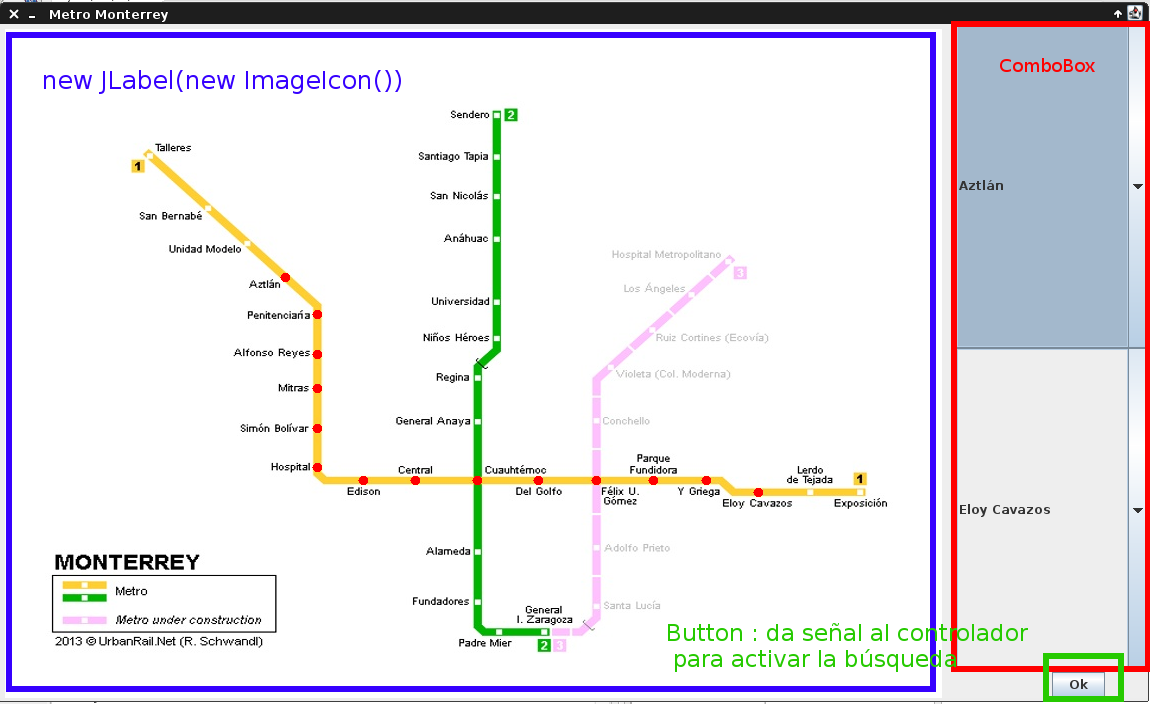
\includegraphics[width=0.9\textwidth]{images/interface.png}
\end{frame}

\begin{frame}{Problemas encontrados}
\begin{itemize}
\item Hacer
\item Tomar distancias aéreas
\item Las resources en la exportación del proyecto
\item Organización en el grupo
\end{itemize}
\end{frame}

\begin{frame}{Demo}
\end{frame}

\end{document}